\section{Лекция 7. Уравнения в полных дифференциалах}
\noeqref{eq:l7_inc_1d, eq:l7_diff_1d, eq:l7_inc_2d, eq:l7_diff_2d}
\noeqref{eq:l7_exact_ode, eq:l7_exact_du, eq:l7_first_int, eq:l7_criterion}
\noeqref{eq:l7_sys_u, eq:l7_int_p, eq:l7_eq_g, eq:l7_ex1, eq:l7_f186}

\begin{flushright}
    19.10.26
\end{flushright}

\subsection{Понятие полного дифференциала функции}

Прежде чем переходить к новому классу дифференциальных уравнений 1-го порядка,
напомним понятие дифференциала для функций одной и двух независимых переменных.

\begin{definition}
    Пусть функция одной переменной $f(x)$ определена в окрестности точки $x$.
    Она называется \textdef{дифференцируемой} в точке $x$, если её приращение
    $\Delta f = f(x + \Delta x) - f(x)$ можно представить в виде:
    \begin{equation} \label{eq:l7_inc_1d}
        \Delta f = f(x + \Delta x) - f(x) = A \Delta x + o\left(\abs{\Delta x}\right)
        \quad \text{при } \Delta x \to 0, \tag{1}
    \end{equation}
    где $A \in \R$ — константа, не зависящая от $\Delta x$. Главная линейная
    часть приращения функции называется её \textdef{дифференциалом}
    (полагая $dx = \Delta x$):
    \begin{equation} \label{eq:l7_diff_1d}
        df = A \, dx = f'(x) \, dx. \tag{2}
    \end{equation}
\end{definition}

Аналогичная конструкция вводится для функции двух переменных $f(x, y)$,
определённой в некоторой открытой области $D \subset \R^2$.

\begin{definition}
    Функция $f(x, y)$ называется \textdef{дифференцируемой} в точке
    $(x, y) \in D$, если её полное приращение представимо в виде:
    \begin{equation} \label{eq:l7_inc_2d}
        \Delta f = f(x + \Delta x, y + \Delta y) - f(x, y) =
        A \Delta x + B \Delta y +
        o\left(\sqrt{(\Delta x)^2 + (\Delta y)^2}\right) \tag{3}
    \end{equation}
    при $\sqrt{(\Delta x)^2 + (\Delta y)^2} \to 0$, где числа $A$ и $B$ не
    зависят от $\Delta x$ и $\Delta y$. Главная линейная относительно
    приращений $dx = \Delta x$ и $dy = \Delta y$ часть приращения \eqref{eq:l7_inc_2d}
    называется \textdef{полным дифференциалом} функции $f(x, y)$:
    \begin{equation} \label{eq:l7_diff_2d}
        df = A \, dx + B \, dy =
        \frac{\partial f}{\partial x} \, dx +
        \frac{\partial f}{\partial y} \, dy. \tag{4}
    \end{equation}
\end{definition}

\begin{remark}
    Если функция $f(x, y)$ непрерывно дифференцируема в области $D$, то есть
    $f \in C^1(D)$ (её частные производные $f'_x, f'_y \in C(D)$), то она
    гарантированно дифференцируема в каждой точке $(x, y) \in D$, а её полный
    дифференциал задаётся формулой \eqref{eq:l7_diff_2d}.
\end{remark}

\subsection{Уравнения в полных дифференциалах и первый интеграл}

Рассмотрим дифференциальное уравнение 1-го порядка, записанное в симметричной
дифференциальной форме в области $D \subset \R^2$:
\begin{equation} \label{eq:l7_exact_ode}
    P(x, y) \, dx + Q(x, y) \, dy = 0, \tag{5}
\end{equation}
где коэффициенты непрерывно дифференцируемы: $P, Q \in C^1(D)$ (то есть
$P, Q, P'_x, P'_y, Q'_x, Q'_y \in C(D)$) и не обращаются в нуль одновременно.

\begin{definition}
    Уравнение \eqref{eq:l7_exact_ode} называется \textdef{уравнением в полных
    дифференциалах} в области $D \subset \R^2$, если существует такая
    непрерывно дифференцируемая функция $u(x, y) \in C^1(D)$ (называемая
    \textdef{потенциалом}), полный дифференциал которой в области $D$
    совпадает с левой частью уравнения \eqref{eq:l7_exact_ode}:
    \begin{equation} \label{eq:l7_exact_du}
        du(x, y) = \frac{\partial u}{\partial x} \, dx +
        \frac{\partial u}{\partial y} \, dy = P(x, y) \, dx + Q(x, y) \, dy.
        \tag{6}
    \end{equation}
\end{definition}

\begin{definition}
    Непостоянная функция $u(x, y) \in C^1(D)$ ($u(x, y) \not\equiv \text{const}$)
    называется \textdef{первым интегралом} (или просто \textdef{интегралом})
    дифференциального уравнения \eqref{eq:l7_exact_ode}, если вдоль любой
    интегральной кривой $y = y(x)$ этого уравнения она сохраняет постоянное
    значение:
    \[
        u(x, y(x)) \equiv C = \text{const}.
    \]
\end{definition}

Если уравнение \eqref{eq:l7_exact_ode} является уравнением в полных
дифференциалах и потенциал $u(x, y)$ найден, то само уравнение переписывается
в виде:
\begin{equation} \label{eq:l7_first_int}
    du(x, y) = 0 \implies u(x, y) = C, \tag{7}
\end{equation}
где соотношение $u(x, y) = C$ задаёт общий интеграл уравнения.

\textbf{Геометрический смысл уравнения в полных дифференциалах:}
Левую часть уравнения \eqref{eq:l7_exact_ode} можно рассматривать как скалярное
произведение векторного поля градиента
$\nabla u(x, y) = \left(\frac{\partial u}{\partial x}, \frac{\partial u}{\partial y}\right) = (P, Q)$
на вектор бесконечно малого смещения $d\mathbf{r} = (dx, dy)$ вдоль
интегральной кривой:
\[
    du = \langle \nabla u, d\mathbf{r} \rangle = P \, dx + Q \, dy = 0.
\]
Следовательно, в каждой точке плоскости $Oxy$ касательный вектор $(dx, dy)$ к
интегральной кривой ортогонален градиенту $\nabla u(x, y)$, а сами интегральные
кривые представляют собой \textdef{линии уровня} $u(x, y) = C$ потенциальной
поверхности $z = u(x, y)$.

\begin{figure}[H]
    \centering
    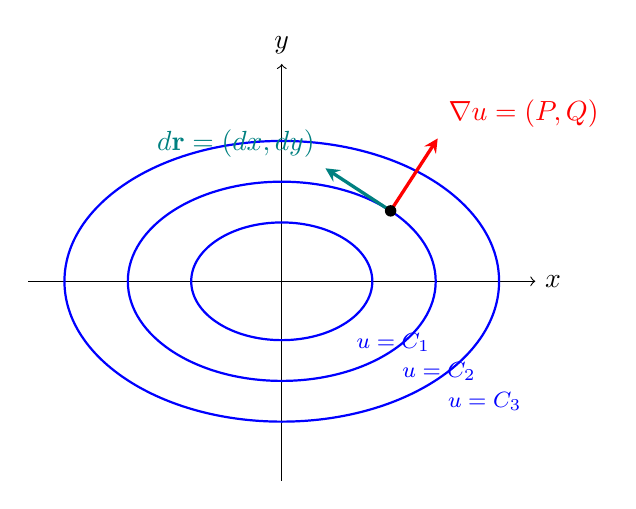
\begin{tikzpicture}[scale=1.15]
        % Оси координат
        \draw[->] (-2.8, 0) -- (2.8, 0) node[right] {$x$};
        \draw[->] (0, -2.2) -- (0, 2.4) node[above] {$y$};

        % Линии уровня u(x, y) = C (семейство эллипсов)
        \foreach \rx/\ry/\lbl in {1.0/0.65/C_1, 1.7/1.1/C_2, 2.4/1.55/C_3} {
            \draw[blue, thick] (0, 0) ellipse ({\rx} and {\ry});
            \node[blue, below right] at ({\rx*0.72}, {-\ry*0.72})
                {\footnotesize $u = \lbl$};
        }

        % Выделенная точка на линии уровня C_2
        \pgfmathsetmacro{\ang}{45}
        \pgfmathsetmacro{\px}{1.7 * cos(\ang)}
        \pgfmathsetmacro{\py}{1.1 * sin(\ang)}

        % Касательный вектор dr = (dx, dy) и вектор градиента (P, Q)
        \draw[teal, very thick, -stealth] (\px, \py)
            -- (\px - 0.72, \py + 0.47)
            node[above left] {$d\mathbf{r} = (dx, dy)$};
        \draw[red, very thick, -stealth] (\px, \py)
            -- (\px + 0.52, \py + 0.80)
            node[above right] {$\nabla u = (P, Q)$};

        % Знак прямого угла
        \fill[black] (\px, \py) circle (1.8pt);
    \end{tikzpicture}
    \caption{Геометрическая интерпретация: интегральные кривые совпадают с
    линиями уровня $u(x, y) = C$, а вектор градиента $\nabla u = (P, Q)$ всюду
    ортогонален касательному вектору $d\mathbf{r} = (dx, dy)$.}
\end{figure}

\subsection{Критерий полного дифференциала}

Возникает естественный вопрос: как по заданным функциям $P(x, y)$ и $Q(x, y)$
определить, является ли выражение $P \, dx + Q \, dy$ полным дифференциалом
некоторой функции $u(x, y)$?

\begin{definition}
    Область $D \subset \R^2$ называется \textdef{односвязной}, если любой
    замкнутый непрерывный контур $\gamma \subset D$ можно непрерывно
    деформировать (стянуть) в точку, принадлежащую области $D$, не выходя за
    пределы $D$ (наглядно: область не имеет «дыр» и выколотых точек).
\end{definition}

\begin{figure}[H]
    \centering
    \begin{tikzpicture}[scale=1.05]
        % --- Панель 1: Односвязная область ---
        \begin{scope}[shift={(-3.2, 0)}]
            \filldraw[fill=blue!8, draw=blue, thick]
                plot[smooth cycle, tension=0.8]
                coordinates {(-1.6, -0.8) (-0.5, -1.3) (1.4, -0.9)
                             (1.7, 0.7) (0.3, 1.4) (-1.4, 0.9)};
            \draw[red, thick, dashed] (0.1, 0.1) ellipse (0.85 and 0.55);
            \draw[red, thick, dashed] (0.1, 0.1) ellipse (0.45 and 0.28);
            \fill[red] (0.1, 0.1) circle (2pt) node[above] {$M_0$};
            \node at (-1.1, 0.6) {$D_1$};
            \node[below] at (0, -1.6) {\textbf{а)} Односвязная область};
        \end{scope}

        % --- Панель 2: Неодносвязная область (с дыркой) ---
        \begin{scope}[shift={(3.2, 0)}]
            \filldraw[fill=blue!8, draw=blue, thick]
                plot[smooth cycle, tension=0.8]
                coordinates {(-1.6, -0.8) (-0.5, -1.3) (1.4, -0.9)
                             (1.7, 0.7) (0.3, 1.4) (-1.4, 0.9)};
            % Вырезанная "дырка"
            \filldraw[fill=white, draw=blue, thick]
                (0.1, 0.1) circle (0.45);
            \draw[red, thick] (0.1, 0.1) circle (0.8);
            \node[red, right] at (0.9, 0.1) {$\gamma$};
            \node at (-1.1, 0.6) {$D_2$};
            \node[below] at (0, -1.6) {\textbf{б)} Неодносвязная область};
        \end{scope}
    \end{tikzpicture}
    \caption{Топология области $D \subset \R^2$: а) в односвязной области $D_1$
    любой замкнутый контур стягивается в точку $M_0 \in D_1$; б) в
    неодносвязной области $D_2$ контур $\gamma$, охватывающий «дыру», нельзя
    стянуть в точку внутри $D_2$.}
\end{figure}

\begin{theorem}[\textbf{Критерий уравнения в полных дифференциалах}]
    \label{thm:l7_criterion}
    Пусть $D \subset \R^2$ — односвязная область и функции
    $P, Q \in C^1(D)$. Дифференциальная форма $P(x, y) \, dx + Q(x, y) \, dy$
    является полным дифференциалом некоторой функции $u(x, y) \in C^2(D)$ в
    области $D$ тогда и только тогда, когда в каждой точке $(x, y) \in D$
    выполняется тождество:
    \begin{equation} \label{eq:l7_criterion}
        \frac{\partial Q}{\partial x} = \frac{\partial P}{\partial y}. \tag{8}
    \end{equation}
\end{theorem}

\begin{proof}[Доказательство необходимости]~\\
    \begin{quote}
        Предположим, что выражение $P \, dx + Q \, dy$ является полным
        дифференциалом некоторой функции $u(x, y) \in C^2(D)$. Тогда из
        равенства дифференциалов \eqref{eq:l7_exact_du} в силу независимости
        $dx$ и $dy$ следует система:
        \[
            \frac{\partial u}{\partial x} = P(x, y), \qquad
            \frac{\partial u}{\partial y} = Q(x, y).
        \]
        Продифференцируем первое равенство по переменной $y$, а второе — по
        переменной $x$:
        \[
            \frac{\partial P}{\partial y} =
            \frac{\partial^2 u}{\partial y \partial x}, \qquad
            \frac{\partial Q}{\partial x} =
            \frac{\partial^2 u}{\partial x \partial y}.
        \]
        Поскольку $P, Q \in C^1(D)$, смешанные производные второго порядка
        функции $u(x, y)$ непрерывны в области $D$. По теореме Шварца о
        равенстве смешанных частных производных имеем
        $\frac{\partial^2 u}{\partial y \partial x} = \frac{\partial^2 u}{\partial x \partial y}$,
        откуда немедленно следует условие \eqref{eq:l7_criterion}:
        $\frac{\partial P}{\partial y} = \frac{\partial Q}{\partial x}$.

        \textit{Замечание о достаточности:} В обратную сторону в односвязной
        области $D$ условие \eqref{eq:l7_criterion} по формуле Грина гарантирует
        независимость криволинейного интеграла $\int P \, dx + Q \, dy$ от пути
        интегрирования, что позволяет явно построить функцию $u(x, y)$
        интегрированием по координатам.
    \end{quote}
\end{proof}

\subsection{Методы решения уравнений в полных дифференциалах}

\subsubsection{Метод I. Непосредственное выделение дифференциалов («метод пристального взгляда»)}

В ряде простых случаев левую часть уравнения удаётся сразу свернуть в полный
дифференциал с помощью таблицы основных дифференциалов:
\begin{align*}
    x \, dy + y \, dx &= d(x y), &
    x \, dx \pm y \, dy &= \frac{1}{2} d\left(x^2 \pm y^2\right), \\
    \frac{x \, dy - y \, dx}{x^2} &= d\left(\frac{y}{x}\right), &
    \frac{x \, dy - y \, dx}{x^2 + y^2} &= d\left(\arctan \frac{y}{x}\right).
\end{align*}

\begin{example}
    Решить уравнение $y \, dx + x \, dy = 0$ методом выделения полного
    дифференциала.

    \begin{proof}[Решение]~\\
        \begin{quote}
            Замечаем, что левая часть представляет собой дифференциал
            произведения:
            \[
                y \, dx + x \, dy = 0 \implies d(x y) = 0 \implies x y = C.
            \]
        \end{quote}
    \end{proof}
\end{example}

\subsubsection{Метод II. Общий алгоритм восстановления функции двух переменных по её полному дифференциалу}

Если свернуть дифференциал устно затруднительно, применяется универсальный
аналитический алгоритм.

\begin{proof}[Алгоритм восстановления потенциала $u(x, y)$]~\\
    \begin{quote}
        \textbf{Шаг 1.} Проверяем выполнение критерия \eqref{eq:l7_criterion}:
        $\frac{\partial Q}{\partial x} = \frac{\partial P}{\partial y}$. Если
        тождество выполнено, то существует функция $u(x, y)$, удовлетворяющая
        системе уравнений в частных производных:
        \begin{equation} \label{eq:l7_sys_u}
            \begin{cases}
                \dfrac{\partial u}{\partial x} = P(x, y), \\[2mm]
                \dfrac{\partial u}{\partial y} = Q(x, y).
            \end{cases} \tag{9}
        \end{equation}

        \textbf{Шаг 2.} Интегрируем первое уравнение системы \eqref{eq:l7_sys_u}
        по переменной $x$, считая переменную $y$ константой. При этом роль
        произвольной постоянной интегрирования играет неизвестная гладкая
        функция $g(y)$, зависящая от $y$:
        \begin{equation} \label{eq:l7_int_p}
            u(x, y) = \int P(x, y) \, dx + g(y). \tag{10}
        \end{equation}

        \textbf{Шаг 3.} Подставляем выражение \eqref{eq:l7_int_p} во второе
        уравнение системы \eqref{eq:l7_sys_u}, дифференцируя его по $y$:
        \begin{equation} \label{eq:l7_eq_g}
            \frac{\partial}{\partial y} \left(\int P(x, y) \, dx + g(y)\right)
            = Q(x, y) \implies
            \frac{\partial}{\partial y} \left(\int P(x, y) \, dx\right) + g'(y)
            = Q(x, y). \tag{11}
        \end{equation}
        В силу условия $\frac{\partial P}{\partial y} = \frac{\partial Q}{\partial x}$
        все слагаемые, содержащие переменную $x$, в левой и правой частях
        \eqref{eq:l7_eq_g} взаимно уничтожаются. Отсюда находим $g'(y)$ и
        интегрированием восстанавливаем $g(y)$.

        \textbf{Шаг 4.} Подставляем найденную функцию $g(y)$ в формулу
        \eqref{eq:l7_int_p} и записываем общий интеграл уравнения в виде
        $u(x, y) = C$.
    \end{quote}
\end{proof}

\begin{example}
    Решить уравнение общим методом восстановления потенциала:
    \begin{equation} \label{eq:l7_ex1}
        y \, dx + x \, dy = 0. \tag{12}
    \end{equation}

    \begin{proof}[Решение]~\\
        \begin{quote}
            Здесь $P(x, y) = y$ и $Q(x, y) = x$. Проверим условие полного
            дифференциала \eqref{eq:l7_criterion}:
            \[
                \frac{\partial Q}{\partial x} = \frac{\partial (x)}{\partial x}
                = 1, \qquad
                \frac{\partial P}{\partial y} = \frac{\partial (y)}{\partial y}
                = 1 \implies
                \frac{\partial Q}{\partial x} = \frac{\partial P}{\partial y}.
            \]
            Следовательно, существует функция $u(x, y)$ такая, что:
            \[
                \begin{cases}
                    u'_x = y, \\
                    u'_y = x.
                \end{cases}
            \]
            Интегрируем первое уравнение по $x$:
            \[
                u(x, y) = \int y \, dx = x y + g(y).
            \]
            Дифференцируем полученное выражение по $y$ и приравниваем ко
            второму уравнению системы:
            \[
                u'_y = \frac{\partial}{\partial y} \left(x y + g(y)\right) =
                x + g'(y) = x \implies g'(y) = 0 \implies g(y) = C_1.
            \]
            Таким образом, $u(x, y) = x y + C_1$. Записывая общий интеграл
            $u(x, y) = \tilde{C}$ и объединяя константы $C = \tilde{C} - C_1$,
            получаем семейство гипербол:
            \[
                x y = C.
            \]
        \end{quote}
    \end{proof}
\end{example}

\begin{problem}[Ф.186]
    Решить дифференциальное уравнение:
    \begin{equation} \label{eq:l7_f186}
        2 x y \, dx + \left(x^2 - y^2\right) dy = 0. \tag{13}
    \end{equation}
\end{problem}

\begin{proof}[Решение]~\\
    \begin{quote}
        Выпишем коэффициенты уравнения:
        \[
            P(x, y) = 2 x y, \qquad Q(x, y) = x^2 - y^2.
        \]
        Обе функции принадлежат классу $C^\infty(\R^2)$ на односвязной
        плоскости $\R^2$. Вычислим частные производные для проверки критерия
        \eqref{eq:l7_criterion}:
        \[
            \frac{\partial Q}{\partial x} =
            \frac{\partial \left(x^2 - y^2\right)}{\partial x} = 2x, \qquad
            \frac{\partial P}{\partial y} =
            \frac{\partial (2 x y)}{\partial y} = 2x.
        \]
        Поскольку $\frac{\partial Q}{\partial x} = \frac{\partial P}{\partial y}$
        тождественно на $\R^2$, уравнение \eqref{eq:l7_f186} является уравнением
        в полных дифференциалах.

        Составим систему для нахождения потенциала $u(x, y)$:
        \[
            \begin{cases}
                u'_x = 2 x y, \\
                u'_y = x^2 - y^2.
            \end{cases}
        \]
        Проинтегрируем первое уравнение системы по переменной $x$:
        \[
            u(x, y) = \int 2 x y \, dx = 2 y \int x \, dx = x^2 y + g(y).
        \]
        Продифференцируем найденное представление по переменной $y$ и
        подставим во второе уравнение системы:
        \[
            u'_y = \left(x^2 y + g(y)\right)'_y = x^2 + g'(y) = x^2 - y^2.
        \]
        Сокращая $x^2$ в обеих частях, находим функцию $g(y)$:
        \[
            g'(y) = -y^2 \implies g(y) = -\int y^2 \, dy = -\frac{y^3}{3} + C_1.
        \]
        Подставляя $g(y)$ обратно в выражение для $u(x, y)$, получаем общий
        интеграл уравнения:
        \[
            x^2 y - \frac{y^3}{3} = C.
        \]

        \textbf{Ответ:} $x^2 y - \dfrac{y^3}{3} = C$.
    \end{quote}
\end{proof}

\begin{figure}[H]
    \centering
    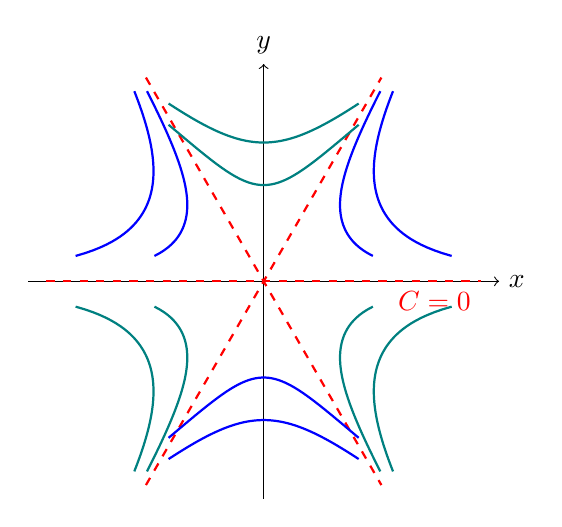
\begin{tikzpicture}[scale=1.15]
        % Оси координат
        \draw[->] (-2.6, 0) -- (2.6, 0) node[right] {$x$};
        \draw[->] (0, -2.4) -- (0, 2.4) node[above] {$y$};

        % Сепаратрисы при C = 0: y = 0 и y = \pm \sqrt{3} x
        \draw[red, thick, dashed] (-2.4, 0) -- (2.4, 0)
            node[below left, red] {$C = 0$};
        \draw[red, thick, dashed] (-1.3, -2.25) -- (1.3, 2.25);
        \draw[red, thick, dashed] (-1.3, 2.25) -- (1.3, -2.25);

        % Линии уровня x^2 = y^2 / 3 + C / y для C > 0 (y > 0)
        \foreach \c in {0.4, 1.2} {
            \draw[blue, thick, domain=0.28:2.1, samples=60]
                plot ({sqrt(\x*\x/3 + \c/\x)}, \x);
            \draw[blue, thick, domain=0.28:2.1, samples=60]
                plot ({-sqrt(\x*\x/3 + \c/\x)}, \x);
            % Нижние ветви при y < 0 для C < 0
            \draw[teal, thick, domain=0.28:2.1, samples=60]
                plot ({sqrt(\x*\x/3 + \c/\x)}, -\x);
            \draw[teal, thick, domain=0.28:2.1, samples=60]
                plot ({-sqrt(\x*\x/3 + \c/\x)}, -\x);
        }

        % Боковые ветви в секторах |y| > \sqrt{3}|x|
        \foreach \c in {0.4, 1.2} {
            \draw[teal, thick, domain=-1.05:1.05, samples=60]
                plot (\x, {(3*\c + 3*\x*\x*1.2)^(1/3)});
            \draw[blue, thick, domain=-1.05:1.05, samples=60]
                plot (\x, {-(3*\c + 3*\x*\x*1.2)^(1/3)});
        }
    \end{tikzpicture}
    \caption{Семейство интегральных кривых (линий уровня первого интеграла
    $x^2 y - y^3/3 = C$) для задачи Ф.186: при $C = 0$ линии уровня распадаются
    на три прямые $y = 0$ и $y = \pm\sqrt{3} x$, проходящие через седловую
    точку $(0, 0)$.}
\end{figure}